\section{Results and Discussion} \label{sec:results}

\begin{figure}
  \centering
  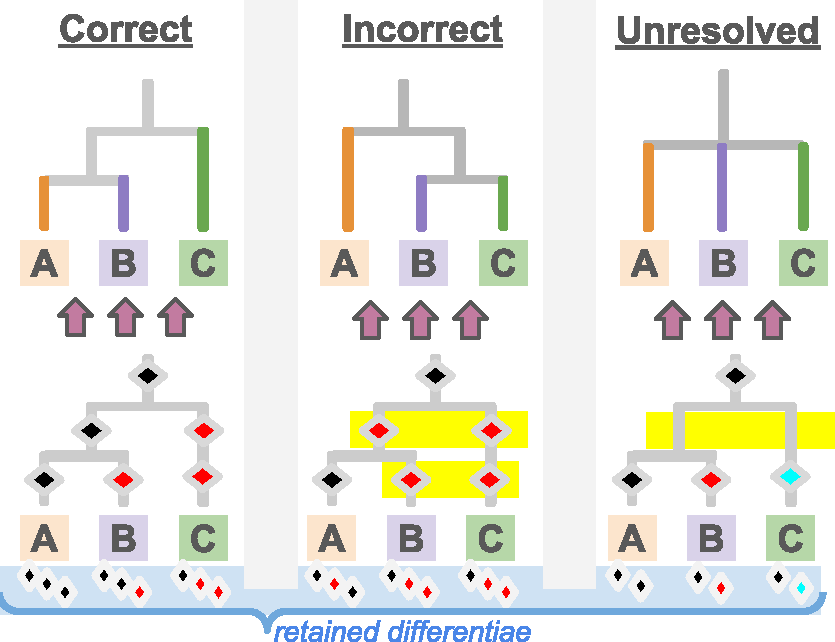
\includegraphics[width=\linewidth]{img/hstrat-failure-modes}
  \caption{%
    \textbf{Differentia structure and reconstruction outcomes.}
    Illustration depicts possible outcomes of reconstruction from hereditary stratigraphy differentia (diamonds) generated and inherited along a two-branch phylogeny (panel bottoms) and resulting reconstruction outcomes (panel tops).
    Diamond placement indicates when differentia were gained and color represents each differentiae's randomly-generated value.
    Diamonds below phylogeny tips summarize inherited hereditary stratigraph record of that taxon.
    \textbf{\textit{Correct reconstruction}} (left panel) occurs when differentia intersperse branching events and differentia value collisions do not occur.
    \textbf{\textit{Incorrect reconstruction}} (center panel) occurs when differentia collisions make unrelated taxa falsely appear related (yellow highlights).
    \textbf{\textit{Unresolved reconstruction}} (i.e., false polytomies; right panel) occurs when differentia do not intersperse branching events but collisions do not occur.
    Note that unresolved reconstructions require differentia size larger than one bit (in order to support $>2$ differentia values), except in the case where more than two differentia records are entirely identical.
  }
  \label{fig:hstrat-failure-modes}
\end{figure}


\subsection{Surface vs. Column} \label{sec:surface-vs-column}

\begin{figure*}
  \centering
  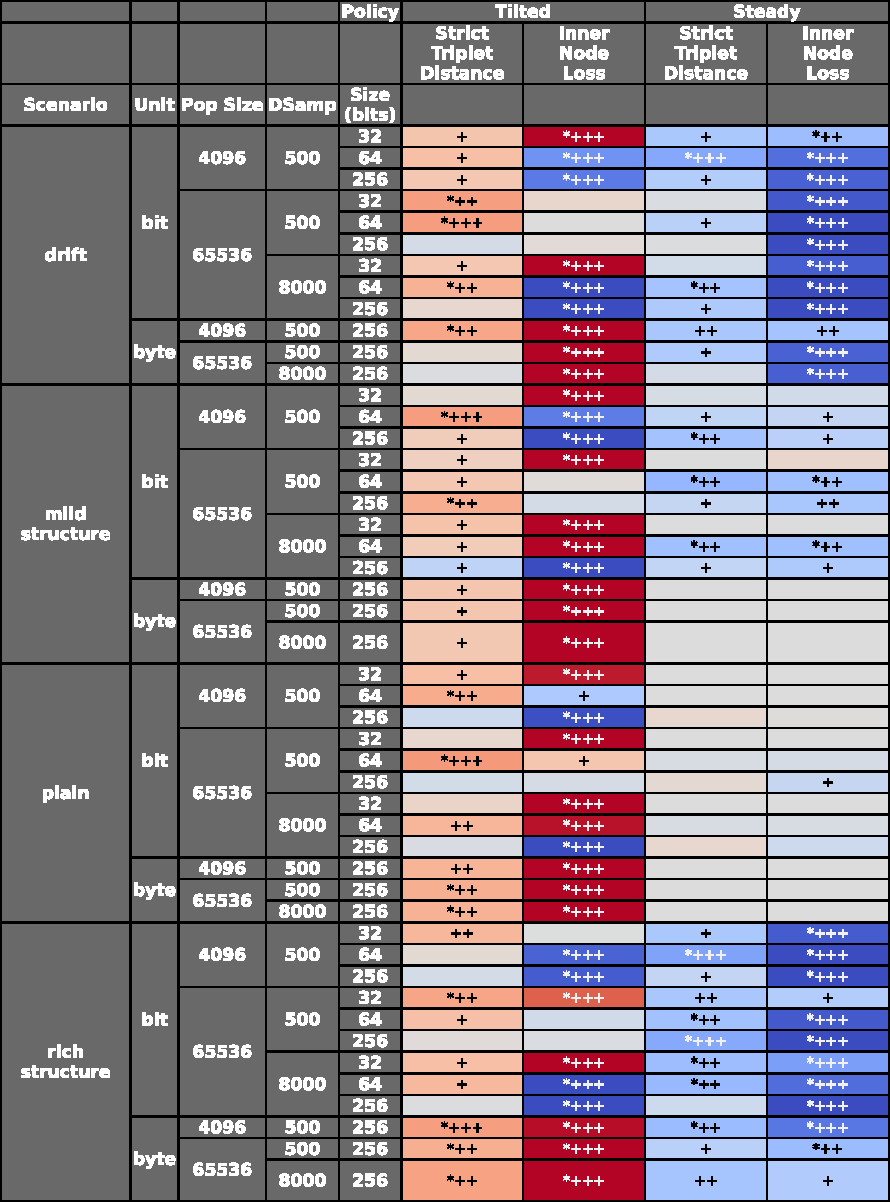
\includegraphics[width=0.9\textwidth]{binder/binder/surf-vs-col/outplots/surf-vs-col-table}
  \caption{%
   \textbf{Comparison of reconstruction quality from column- and surface-based annotations.}
   \footnotesize
    Color coding reflects non-parametric comparison between quality measure values, with red indicating superior surface performance and blue indicating superior column performance.
    Left column shows tilted retention policies, and right column shows steady retention policies.
    In cell annotations, +'s indicate small, medium, and large effect sizes using the Cliff's delta statistic and *'s indicate statistical significance at $\alpha = 0.05$ via Mann-Whitney U test.
  }
  \label{fig:col-vs-surf}
\end{figure*}

\begin{itemize}
    \item surf steady worse than col steady
    \item surf tilted better than col tilted
\end{itemize}

From this point onwards, only surf algorithms!!!

\subsection{Steady vs. Tilted} \label{sec:steady-vs-tilted}
\begin{itemize}
    \item steady worse than tilted
    \item hybrid similar to tilted
\end{itemize}

\begin{figure*}
  \centering
  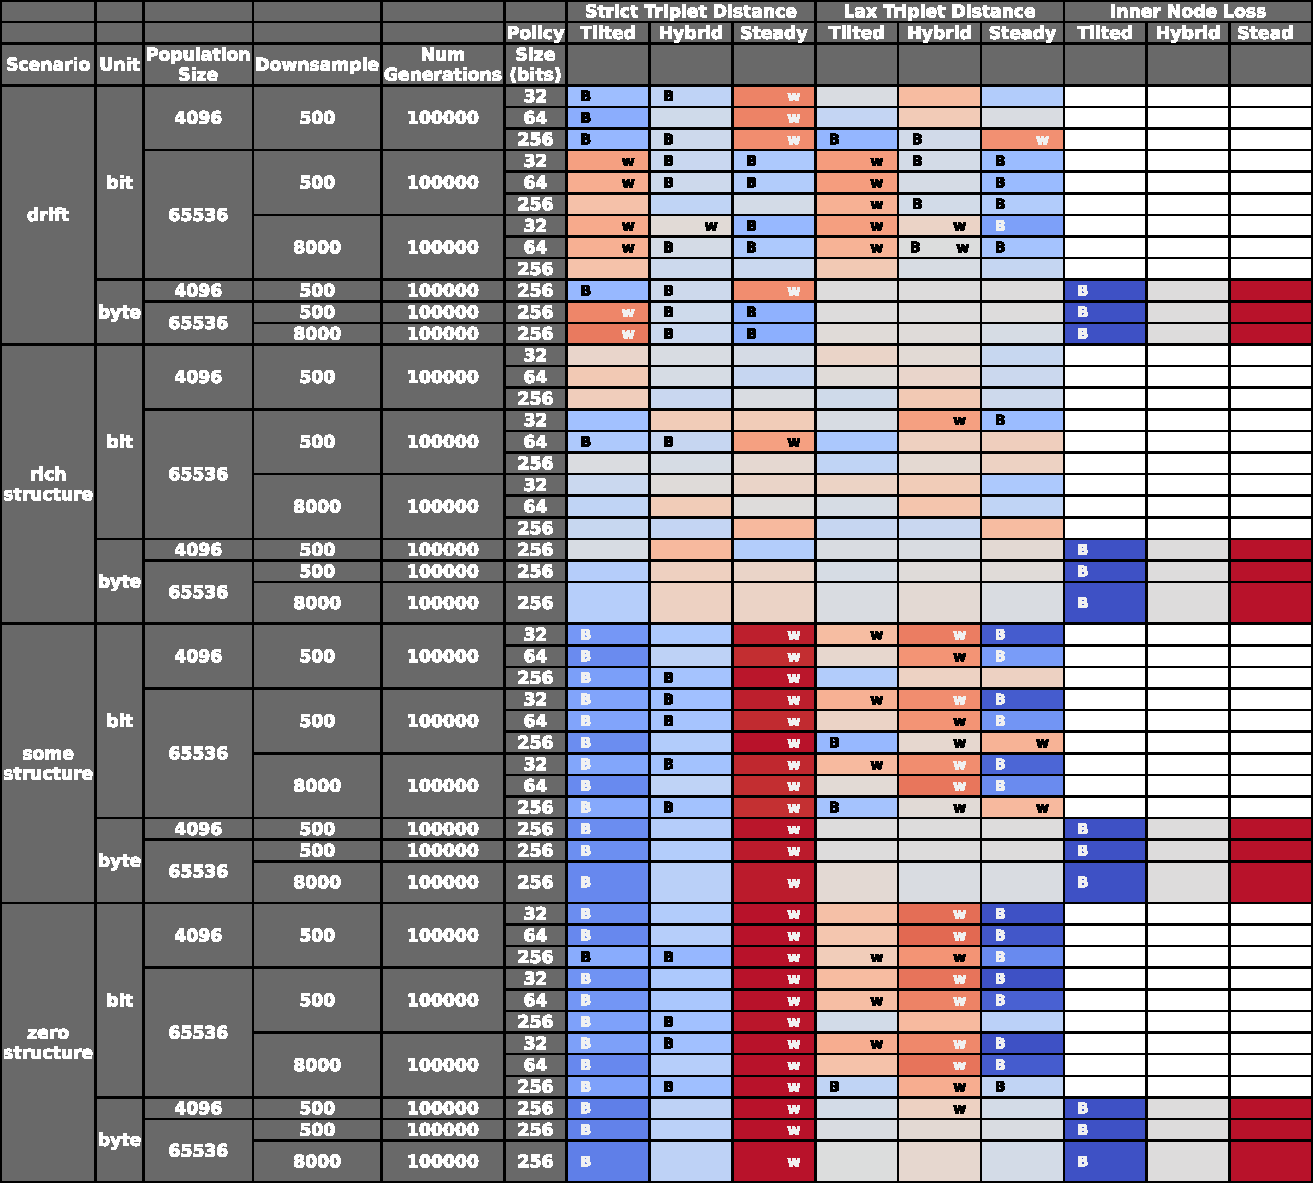
\includegraphics[width=\textwidth]{binder/binder/steady-vs-tilted/outplots/steady-vs-tilted-value}
  \caption{%
    \textbf{Comparison of reconstruction qualities under different differentia retention strategies.}
    \footnotesize
    Steady retention experiments used column-based implementation; tilted and hybrid retention experiments used surface-based implementation.
    For heatmap charts, B's indicate significantly best and w's significantly worst.
    Heatmap coloring is nonparametric mean rank among the three algorithms, with blue best and red worst.
  }
  \label{fig:steady-vs-tilted}
\end{figure*}


\subsection{Why is Steady Bad? What Type of Error is Made?} \label{sec:error-analysis}
\begin{itemize}
    \item inner node loss from boxplot
    \item then, it's coming from recent nodes: node density vs. time histogram joyplot
    \item then, and that causes error: show error category (correct/wrong/unsure) vs. time stacked bar plot
\end{itemize}

From this point onwards, only surface-tilted (maybe also tilted-hybrid?) algorithm(s)!!!!

\subsection{Why are we seeing error? What can we do about it?} \label{sec:error-uncertainty}

mechanism of error: you have a lineage that diverges three ways between checkpoints (maybe make a figure of this); the two LEAST related happen to collide at the next checkpoint --- therefore, it looks like they're most related even though they're not.

sidebar: we can use differentia size to trade off between error and reconstruction accuracy; using 1 byte differentia essentially drives error to zero (but introduces uncertainty i.e., more polytomies in reconstruction)

\subsection{Does it Scale?} \label{sec:scaling}

\begin{figure*}
  \centering
  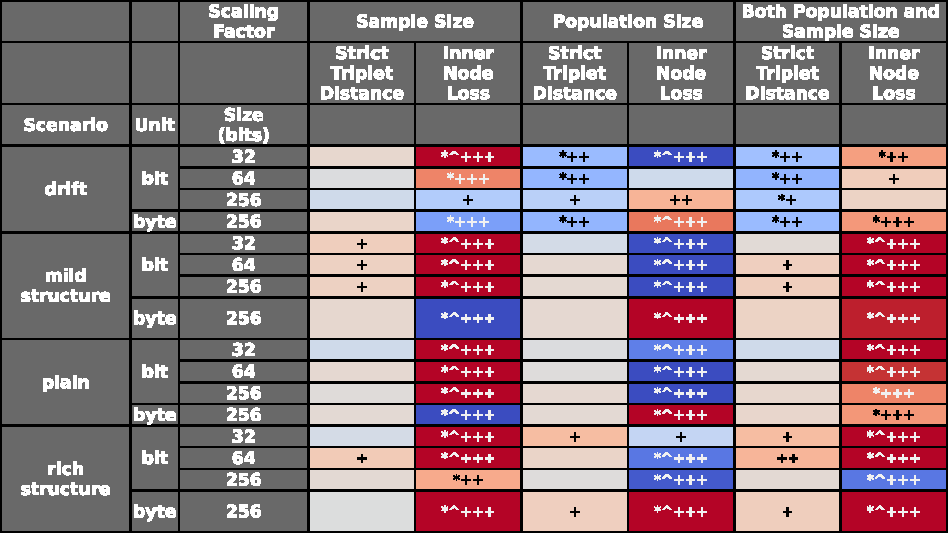
\includegraphics[width=\textwidth]{binder/binder/dsamp-popsize-scale/outplots/dsamp-popsize-scale-hybrid.pdf}
  \caption{%
    Bigger downsample (8000) (red) vs. smaller downsample (500) (blue) performance.
    For heatmap charts, +'s indicate small, medium, and large effect sizes using the Cliff's delta statistic and *'s indicate statistical significance at $\alpha = 0.05$ via Mann-Whitney U test.
  }
  \label{fig:popsize-scale-hybrid}
\end{figure*}

\begin{figure*}
  \centering
  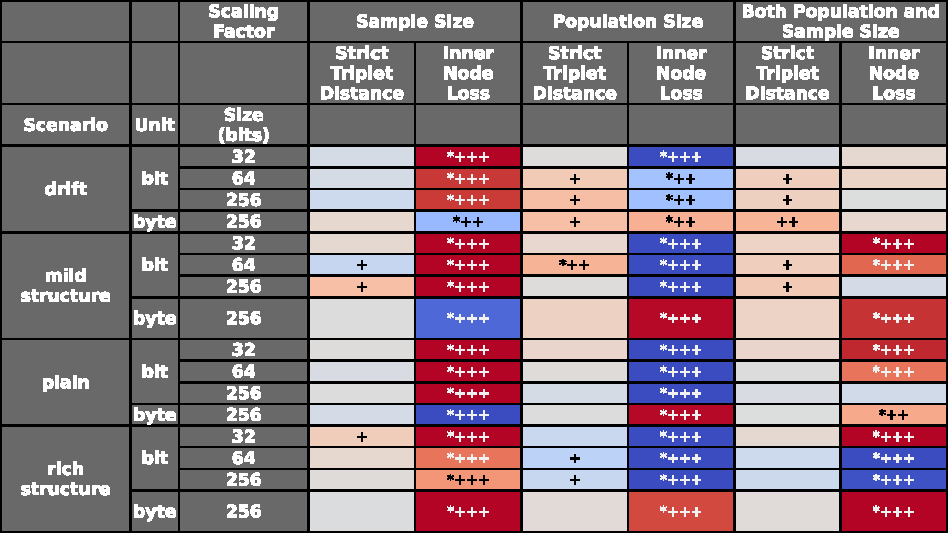
\includegraphics[width=\textwidth]{binder/binder/dsamp-popsize-scale/outplots/dsamp-popsize-scale-tilted.pdf}
  \caption{%
   \textbf{Comparison of reconstruction quality between small and large downsample and population sizes under tilted retention policy.}
    First column considers sample size in isolation, second column considers scaling population size in isolation, and third column considers scaling population and sample size together.
    Color coding reflects non-parametric comparison between quality measure values, with red indicating degraded reconstruction quality at larger scale and blue indicating improved reconstruction quality at larger scale.
    Bigger downsample size is 8,000 taxa and smaller downsample size is 500 taxa.
    Bigger population size is 65,536 and smaller population size is 4,096.
    Experiments used tilted retention policy with surface-based implementation.
    In cell annotations, +'s indicate small, medium, and large effect sizes using the Cliff's delta statistic and *'s indicate statistical significance at $\alpha = 0.05$ via Mann-Whitney U test.
  }
  \label{fig:dsamp-popsize-scale-tilted}
\end{figure*}


\begin{itemize}
    \item show reconstruction error and inner node count vs. pop size (error does not increase with pop size at fixed sample size)
    \item show reconst error/inner node count vs. time (error does not increase with time at fixed sample size)
    \item show reconst error/inner node count vs. sample size (error increases with sample size)
    \item show reconst error/inner node count vs. bit size at large sample (we can reduce the error for large sample size by increasing bit size)
\end{itemize}
